\documentclass[a4paper,10pt,conference]{ieeeconf}

\IEEEoverridecommandlockouts
\overrideIEEEmargins

\usepackage{amsmath}
\usepackage{balance}
\usepackage{booktabs}
\usepackage{graphicx}
\usepackage[hidelinks]{hyperref}
\usepackage{microtype}

% generated by contract-validation aggregate; data_hash=7db98d2efebb442b6f6d8a57019513dd1b6d1319ed30c5ffdcdc94d96e589aa9
\newcommand{\CVMTotalRows}{103}
\newcommand{\CVMPlannedRuns}{0}
\newcommand{\CVMAttemptedRuns}{79}
\newcommand{\CVMCompletedRuns}{79}
\newcommand{\CVMSyntheticCompletedRuns}{55}
\newcommand{\CVMClosedLoopCompletedRuns}{24}
\newcommand{\CVMClosedLoopAuditValidRuns}{18}
\newcommand{\CVMClosedLoopMetricRows}{24}
\newcommand{\CVMFullContractCompletedRuns}{18}
\newcommand{\CVMFullContractAuditValidRuns}{18}
\newcommand{\CVMValidFullContractFalseBlockedRuns}{0}
\newcommand{\CVMValidFullContractFalseBlockDenominator}{18}
\newcommand{\CVMClosedLoopSceneCount}{6}
\newcommand{\CVMRequiredScenarioCategoryCount}{6}
\newcommand{\CVMVerifiedRequiredScenarioCategoryCount}{0}
\newcommand{\CVMUnclassifiedClosedLoopSceneCount}{6}
\newcommand{\CVMScenarioCategoryCoverageClaimed}{0}
\newcommand{\CVMContractValidClosedLoopRows}{18}
\newcommand{\CVMIntegrationInvalidClosedLoopRows}{6}
\newcommand{\CVMClaimValidPolicyBenchmarkRows}{0}
\newcommand{\CVMPolicyBehaviorAttributableRows}{18}
\newcommand{\CVMPolicyFailureAttributableRows}{0}
\newcommand{\CVMIntegrationFailureAttributableRows}{24}
\newcommand{\CVMDiagnosticNotPolicyRows}{61}
\newcommand{\CVMNonPolicyAttributedRows}{85}
\newcommand{\CVMSyntheticDiagnosticRows}{55}
\newcommand{\CVMPublicCoreRows}{12}
\newcommand{\CVMPublicCoreCompletedRuns}{12}
\newcommand{\CVMPublicCoreAttemptedRuns}{12}
\newcommand{\CVMPublicCoreAuditValidRuns}{12}
\newcommand{\CVMPublicCoreBlockedRows}{0}
\newcommand{\CVMOptionalGatedRows}{24}
\newcommand{\CVMOptionalGatedBlockedRows}{24}
\newcommand{\CVMDirectActorRows}{24}
\newcommand{\CVMDirectActorBlockedRows}{24}
\newcommand{\CVMSemanticAblationCompletedPairs}{6}
\newcommand{\CVMSemanticAblationMetricPairs}{6}
\newcommand{\CVMCommandProxyCompletedRuns}{6}
\newcommand{\CVMCommandProxyRejectedRuns}{6}
\newcommand{\CVMNaiveWrapperMetricRuns}{6}
\newcommand{\CVMNaiveInvalidAcceptedRuns}{6}
\newcommand{\CVMContractInvalidRejectedRuns}{6}
\newcommand{\CVMContractInvalidRejectionDenominator}{6}
\newcommand{\CVMAttributionImprovementInvalidRows}{6}
\newcommand{\CVMSemanticProgressDeltaMean}{-0.082}
\newcommand{\CVMSemanticProgressRelDeltaMean}{-0.018}
\newcommand{\CVMSemanticOffroadDeltaMean}{0.000}
\newcommand{\CVMSemanticCollisionAnyDeltaMean}{0.000}
\newcommand{\CVMSemanticPlanDeviationDeltaMean}{0.035}
\newcommand{\CVMClosedLoopCollisionAnyMean}{0.833}
\newcommand{\CVMClosedLoopOffroadMean}{0.000}
\newcommand{\CVMClosedLoopProgressMean}{0.394}
\newcommand{\CVMFailedRuns}{0}
\newcommand{\CVMBlockedRuns}{24}
\newcommand{\CVMSyntheticRuns}{55}
\newcommand{\CVMCoreRows}{18}
\newcommand{\CVMSemanticRows}{12}
\newcommand{\CVMTemporalRows}{18}
\newcommand{\CVMLifecycleRows}{40}
\newcommand{\CVMFaultRows}{15}
\newcommand{\CVMLifecycleFullSurvived}{20}
\newcommand{\CVMLifecycleFullTotal}{20}
\newcommand{\CVMLifecycleStrictSurvived}{0}
\newcommand{\CVMLifecycleStrictTotal}{20}
\newcommand{\CVMFaultDetected}{15}
\newcommand{\CVMFaultLocalized}{15}
\newcommand{\CVMFaultTotal}{15}


\title{\LARGE \bf WOD2Sim: Separating Integration Failures from Policy Failures in Closed-Loop Driving Simulation}

\author{Alba Maria Tellez Fernandez%
\thanks{Alba Maria Tellez Fernandez is an Independent Researcher.
Email: amtellezfernandez@gmail.com.}%
}

\hypersetup{
  pdftitle={WOD2Sim: Separating Integration Failures from Policy Failures in Closed-Loop Driving Simulation},
  pdfauthor={Alba Maria Tellez Fernandez},
  pdfsubject={WOD2Sim integration-failure attribution paper}
}

\begin{document}
\maketitle
\thispagestyle{empty}
\pagestyle{empty}

\begin{abstract}
Closed-loop driving evaluation can misattribute degraded rollout metrics to policy
quality when the simulator boundary drops route geometry, changes timing assumptions,
or produces incomplete evidence. WOD2Sim is a contract-auditing layer between Waymo
Open Dataset (WOD)-style trajectory-policy interfaces and AlpaSim external
drivers. It validates semantic, temporal, lifecycle, deployment, and evidence
contracts before a rollout is admitted as policy-behavior evidence. We evaluate the
public dependency-light path on \CVMClosedLoopSceneCount{} locally available scenes.
All \CVMPublicCoreCompletedRuns{}/\CVMPublicCoreRows{} constant-velocity and
route-following rows complete, of which \CVMPublicCoreAuditValidRuns{} pass route and
sensor audits. Across all matrices, \CVMFullContractAuditValidRuns{}/
\CVMFullContractCompletedRuns{} completed full-contract rollouts are audit-valid. In
a paired route-loss diagnostic, all \CVMStatusOnlyAcceptedRuns{}/
\CVMStatusOnlyAcceptanceDenominator{} command-only rows complete with metrics and pass
a defined status-only baseline, while the contract gate rejects
\CVMContractInvalidRejectedRuns{}/\CVMContractInvalidRejectionDenominator{} because
route geometry is absent. Only \CVMSemanticAblationEligiblePairs{}/
\CVMSemanticAblationCompletedPairs{} pairs are comparison-eligible; their score
deltas are descriptive because each scene has one execution and the simulator seed is
uncontrolled. No learned policy or scenario coverage is evaluated. The contribution
is an auditable failure-attribution method and evidence pipeline, not a policy
benchmark or performance result.
\end{abstract}

\section{Introduction}

Dataset-trained trajectory policies and closed-loop simulators expose different
failure surfaces. A policy designed around the Waymo Open Dataset (WOD)
interface~\cite{sun2020scalability} may assume logged observations, local route
geometry, and a fixed trajectory horizon. A simulator service must also accept
incremental messages, meet the runtime clock, remain alive across session events, and
retain enough evidence to explain a result. AlpaSim exposes this difference through
its external-driver boundary~\cite{alpasim2025}.

A wrapper can therefore make an integration defect look like poor driving. Replacing a
local route polyline with a left/straight/right command removes decision-relevant input,
yet the rollout may still terminate with collision and progress metrics. Timing-grid
mismatches, stale observations, optional import failures, missing assets, and incomplete
manifests create similar confounds. A completed process is not sufficient evidence that
a score characterizes policy behavior.

WOD2Sim treats this as a system-integration and attribution problem. Its contribution is
threefold:
\begin{itemize}
  \item five explicit contracts define when a simulator rollout may be interpreted as
  policy behavior;
  \item an adapter, audit, and artifact pipeline localizes violations and preserves
  completed, blocked, and invalid rows;
  \item a bounded closed-loop evaluation compares a defined status-only acceptance
  baseline with contract-gated attribution while keeping unavailable benchmark work
  outside the claim.
\end{itemize}
The design targets WOD-style trajectory interfaces, but the present evaluation uses
only dependency-light constant-velocity and route-following policies. It does not
evaluate a learned policy.

\subsection{Failure Attribution Rule}

A rollout permits policy-behavior attribution only if its semantic, temporal,
lifecycle, deployment, and evidence contracts pass. A policy-failure attribution
additionally requires a retained failure layer identifying the policy. Otherwise the
row is an integration, precondition, or evidence failure. Thus a missing actor proxy is
not a weak planner, a command-proxy route is not a poor route-conditioned policy, and an
incomplete audit is not a collision result. This rule permits policy behavior to be
examined after validation; it does not declare every degraded metric a policy failure.

\section{Contract-Gated Integration}

Table~\ref{tab:contract-map} maps the five recurring boundary mismatches to enforcement
mechanisms. The \emph{semantic contract} preserves route geometry, ego state, camera
availability, and actor fields at prediction time. A high-level route command may be
diagnostic context, but it cannot substitute for a local polyline. The \emph{temporal
contract} validates horizons and timestamps, anchors interpolation at the current ego
pose, deterministically resamples a finite $N\times2$ trajectory, and recomputes
headings on the runtime grid.

\begin{table}[t]
\centering
\caption{Contracts enforced at the policy/simulator boundary.}
\label{tab:contract-map}
\resizebox{\columnwidth}{!}{% generated by contract-validation aggregate; data_hash=7db98d2efebb442b6f6d8a57019513dd1b6d1319ed30c5ffdcdc94d96e589aa9
\begin{tabular}{llll}
\toprule
Mismatch & Contract & Mechanism & Validation \\
\midrule
Command-only route & Semantic & Preserve route geometry & route-source audit \\
Policy horizon/runtime grid & Temporal & Deterministic resampling & cadence tests \\
Script flow/session service & Lifecycle & Idempotent late-event handling & lifecycle tests \\
Implicit host state & Deployment & Materialized manifests & readiness checks \\
Process exit/evidence & Evidence & Audit-valid summaries & claim gate \\
\bottomrule
\end{tabular}
}
\end{table}

The \emph{lifecycle contract} makes start, active, close, cleanup, duplicate close, and
late events explicit. Recoverable warnings are distinguished from fatal service errors.
The \emph{deployment contract} records launch commands, scene and policy identifiers,
timeout, endpoint, repository state, image identity, and gated inputs. The
\emph{evidence contract} requires unique run identifiers, immutable manifests, terminal
status, route and sensor audits, failed-run retention, and hashes linking generated
paper assets to aggregate rows.

Figure~\ref{fig:architecture} shows the boundary. WOD2Sim reconstructs policy-facing
state, preserves route geometry, resamples outputs, and isolates optional model
discovery. On the runtime side it records deployment and evidence state before a row can
be attributed to policy behavior. Constant-velocity and route-following models form the
public core. Learned-checkpoint and direct actor-aware entry points remain gated when
their checkpoints or scene-matched actor proxies are unavailable.

\begin{figure}[t]
\centering
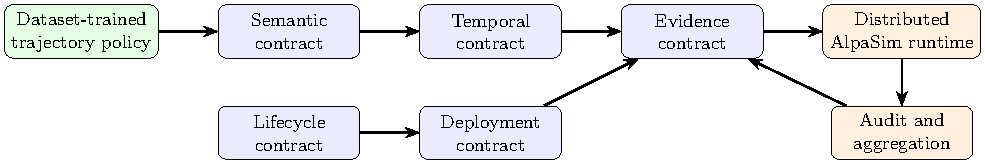
\includegraphics[width=\columnwidth]{figures/system_architecture.pdf}
\caption{Contract gates localize semantic, temporal, lifecycle, deployment, and
evidence failures around the external-driver boundary.}
\label{fig:architecture}
\end{figure}

\section{Implementation and Evidence Pipeline}

\subsection{Policy-Facing Adapter}

The external driver maintains isolated state for each simulator session. Image,
egomotion, route, and close messages update that state; prediction reads one
consistent snapshot rather than reconstructing inputs from process-global variables.
The route converter carries simulator waypoints into the policy input and records their
source. When the explicit command-only diagnostic is selected, it labels the fallback
as \texttt{command\_proxy}; the audit can then reject the row even if the service and
simulator finish normally. Static hazards remain geometry-bearing objects, while
dynamic hazards retain position, motion, heading, and shape fields when the external
interface supplies them. Visibility-risk signals remain diagnostics and do not create
synthetic obstacles.

The temporal adapter maps a source trajectory to runtime times
$t_k=k/f_{\mathrm{run}}$ over the requested horizon. The current ego origin is prepended
before interpolation, source timestamps must be finite and strictly increasing, and the
output must be a finite $N\times2$ array. Matching grids preserve samples; mismatched
grids use deterministic interpolation, after which headings are recomputed from
successive runtime points. Invalid horizons, frequencies, grids, or trajectories fail
the temporal contract rather than reaching vehicle control. These behaviors are
covered by dependency-light tests, but the scene-level temporal comparison remains
blocked and is not reported as a result.

\subsection{Artifact Lineage}

Figure~\ref{fig:pipeline} shows the evidence path. Before launch, the matrix runner
expands a configuration row and materializes its command, environment, scene identity,
policy identity, adapter mode, prerequisite state, and expected route source. A
readiness check distinguishes an executable row from a missing checkpoint, actor
proxy, asset, or runtime dependency. Terminal state is then recorded as completed,
failed, blocked, or planned; non-completed rows are retained rather than removed from
the denominator.

\begin{figure}[t]
\centering
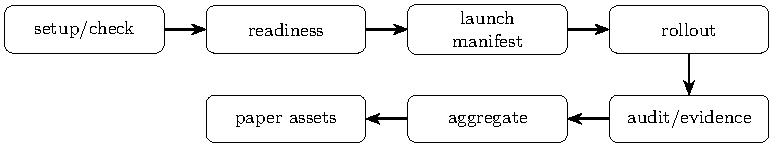
\includegraphics[width=\columnwidth]{figures/evaluation_pipeline.pdf}
\caption{Manifests and audits precede aggregation, so blocked or invalid rows remain
visible and cannot silently become paper results.}
\label{fig:pipeline}
\end{figure}

For completed simulator rows, the audit reconstructs route-source and sensor-freshness
status from retained telemetry and loads behavior metrics without using them to decide
route validity. Aggregation rejects duplicate completed run identifiers, preserves
failure codes, forms paired rows by policy, scene, and execution identifier, and writes
CSV, JSON, LaTeX tables, and vector figures. Generated paper assets carry the aggregate
data hash, and the submission validator compares their values with the JSON source.
This lineage prevents manual table edits from changing a paper result independently of
the row evidence. Restricted sensor frames and licensed scenes are not redistributed;
the public package retains manifests, aggregate metrics, audit fields, and a stable
frame schema. Consequently, artifact lineage is public, but complete replay still
depends on legitimately acquired external scenes and runtime software.

\section{Evaluation Method}

The contract-validation matrix (CVM) contains \CVMTotalRows{} configured rows:
\CVMCoreRows{} core, \CVMSemanticRows{} semantic-ablation, \CVMTemporalRows{}
temporal-ablation, \CVMLifecycleRows{} lifecycle, and \CVMFaultRows{}
fault-injection rows. It completes \CVMCompletedRuns{} rows, including
\CVMClosedLoopCompletedRuns{} simulator rollouts; \CVMBlockedRuns{} optional-extension
rows remain blocked. Lifecycle and fault rows use public service harnesses and are
conformance diagnostics, not simulator-backed effectiveness results.

The public core executes two dependency-light policies over
\CVMClosedLoopSceneCount{} locally cached front-camera scenes. The semantic matrix pairs
full-route and command-only variants of route following on the same scenes. The launcher
does not expose a simulator seed override, so each policy/scene arm has one execution;
the configured seed is provenance metadata rather than proof of deterministic replay.
No authoritative metadata verifies straight, intersection, lane-change, dense-traffic,
occlusion, or merge labels: \CVMUnclassifiedClosedLoopSceneCount{} scenes remain
unclassified and \CVMVerifiedRequiredScenarioCategoryCount{}/
\CVMRequiredScenarioCategoryCount{} required categories are verified.

Completed rows are audited for route source and sensor freshness. For a precise
comparison, define a status-only baseline
\begin{equation}
B_{\mathrm{status}}(r)=
\mathbf{1}[\text{completed}(r)\land\text{metrics}(r)].
\end{equation}
It models the minimal reporting path that scores any completed metric-bearing row; it
is not a separate wrapper implementation or an external competitor. WOD2Sim additionally
requires the five contracts. A semantic pair is comparison-eligible only when both arms
contain metrics, the full-route arm is route-valid and audit-valid, and the
command-only arm is route-invalid and audit-invalid. This criterion excludes one pair
whose nominal full arm also fell back to a command proxy. Metric deltas are therefore
computed on \CVMSemanticAblationEligiblePairs{} pairs, but are not used for an
inferential policy-effect claim.

\section{Results}

Table~\ref{tab:main-results} reports integration status rather than behavior scores.
All \CVMPublicCoreCompletedRuns{}/\CVMPublicCoreRows{} public-core rows complete with
no service crash or blocker; \CVMPublicCoreAuditValidRuns{} are audit-valid. The two
invalid core rows and one invalid semantic full-route row come from the same scene,
where the audit finds late command-proxy fallback. They remain integration/evidence
failures despite successful process completion.

\begin{table}[t]
\centering
\caption{Dependency-light public-core integration status.}
\label{tab:main-results}
\resizebox{\columnwidth}{!}{% generated by contract-validation aggregate; data_hash=7db98d2efebb442b6f6d8a57019513dd1b6d1319ed30c5ffdcdc94d96e589aa9
\begin{tabular}{lllllllll}
\toprule
Public core policy & Rows & Done/att. & Audit & Progress & Coll./off & Lat. p95 & Crash & Blocked \\
\midrule
constant\_velocity & 6 & 6/6 & 6/6 & 0.435 & 0.833/0.000 & -- & 0 & 0 \\
route\_following & 6 & 6/6 & 6/6 & 0.353 & 0.833/0.000 & -- & 0 & 0 \\
\bottomrule
\end{tabular}
}
\end{table}

The central invalidation check is shown in Table~\ref{tab:integration-checks}. All
\CVMStatusOnlyAcceptedRuns{}/\CVMStatusOnlyAcceptanceDenominator{} command-only rows
satisfy $B_{\mathrm{status}}$, whereas WOD2Sim rejects
\CVMContractInvalidRejectedRuns{}/\CVMContractInvalidRejectionDenominator{} as
route-invalid. This demonstrates a classification difference for retained closed-loop
records: completion and metrics alone would admit them, while the semantic contract
prevents policy attribution. It does not demonstrate improved driving or faster fault
diagnosis.

\begin{table}[t]
\centering
\caption{Closed-loop attribution checks from retained rollout and audit artifacts.}
\label{tab:integration-checks}
\resizebox{\columnwidth}{!}{% generated by contract-validation aggregate; data_hash=7db98d2efebb442b6f6d8a57019513dd1b6d1319ed30c5ffdcdc94d96e589aa9
\begin{tabular}{lrr}
\toprule
Closed-loop integration check & Observed & Denom. \\
\midrule
Full-contract audit-valid rollouts & 18 & 18 \\
Valid full-contract rows accepted & 18 & 18 \\
Semantic ablation metric pairs & 6 & 6 \\
Naive command-only route rows with metrics & 6 & 6 \\
Naive invalid route evidence accepted & 6 & 6 \\
Contract invalid route evidence rejected & 6 & 6 \\
Invalid-row attribution improvement & 6 & 6 \\
Policy-behavior diagnostic rows & 18 & 24 \\
Verified scenario categories & 0 & 6 \\
\bottomrule
\end{tabular}
}
\end{table}

Only \CVMSemanticAblationEligiblePairs{}/\CVMSemanticAblationCompletedPairs{} route-loss
pairs satisfy the comparison criterion. Their full-minus-command score deltas have
mixed signs and are descriptive only. With one uncontrolled execution per arm, the
data do not support a systematic route-loss effect or any policy-quality comparison.

\begin{table}[t]
\centering
\caption{Descriptive full-route minus command-only mean deltas over the
\CVMSemanticAblationEligiblePairs{} eligible pairs.}
\label{tab:semantic-deltas}
\begin{tabular}{lr}
\toprule
Metric & Mean delta \\
\midrule
Progress & \CVMSemanticProgressDeltaMean{} \\
Relative progress & \CVMSemanticProgressRelDeltaMean{} \\
Collision-any & \CVMSemanticCollisionAnyDeltaMean{} \\
Off-road & \CVMSemanticOffroadDeltaMean{} \\
Plan deviation & \CVMSemanticPlanDeviationDeltaMean{} \\
\bottomrule
\end{tabular}
\end{table}

Across all retained rows, \CVMPolicyBehaviorAttributableRows{} are
policy-behavior-attributable diagnostics, \CVMPolicyFailureAttributableRows{} are
policy-failure-attributable, and \CVMIntegrationFailureAttributableRows{} are
integration/precondition blockers. The remaining \CVMNonPolicyAttributedRows{} include
blocked, contract-invalid, synthetic, or benchmark-incomplete evidence. These counts
operationalize the distinction: degraded metrics cannot assign policy failure unless
the contracts pass and the retained failure layer is policy.

\subsection{Interpretation}

The experiment validates an attribution mechanism, not a driving intervention. The
positive path shows that \CVMFullContractAuditValidRuns{} completed full-contract rows
meet the recorded route and sensor checks. It does not establish a false-positive rate:
audit-valid rows define the admitted set, and there is no independent oracle labeling
which completed integrations should have passed. For that reason, WOD2Sim reports the
directly observed \CVMFullContractAuditValidRuns{}/\CVMFullContractCompletedRuns{}
audit outcome and makes no ``zero false blocks'' claim.

The negative path asks a narrower counterfactual. If reporting used only terminal status
and metric availability, every command-only row would be admitted. Adding route-source
validity changes the attribution of all \CVMStatusOnlyAcceptedContractRejectedRuns{}
such rows without changing their recorded simulator outcome. This is useful because the
invalid records remain available for debugging while being excluded from policy
evaluation. The gate neither repairs the route nor proves that a valid route would
improve the score; Table~\ref{tab:semantic-deltas} in fact shows small and mixed average
differences across metrics.

Operationally, the same pattern gives each unavailable extension a typed outcome rather
than an omitted experiment. A missing actor proxy or checkpoint is recorded as a
deployment precondition, a command proxy as a semantic violation, and missing audit
state as an evidence violation. This partition makes a future learned-policy study
additive: new rows can be admitted only after their prerequisites and audits pass,
without rewriting the interpretation of the retained invalid or blocked rows.

\section{Related Work and Limitations}

The contracts instantiate interface reasoning for cyber-physical
systems~\cite{sangiovanni2012taming,dealfaro2001interface}. Closed-loop platforms and
benchmarks such as CARLA, nuPlan, Waymax, NAVSIM, and
AlpaSim~\cite{dosovitskiy2017carla,caesar2021nuplan,gulino2023waymax,
dauner2024navsim,alpasim2025} emphasize simulation or planning evaluation. Scenario and
falsification tools such as Scenic, VerifAI, DriveFuzz, and
PlanFuzz~\cite{fremont2019scenic,dreossi2019verifai,kim2022drivefuzz,wan2022planfuzz}
generate or mutate conditions. WOD2Sim is complementary: it asks whether the
policy/simulator boundary preserved the assumptions needed to interpret a rollout.

This distinction is upstream of benchmark metric design. nuPlan and NAVSIM formalize
planning tasks and evaluation measures, while Waymax and CARLA provide controllable
simulation interfaces. AlpaSim provides the external-driver service boundary used here.
Those systems can expose malformed or incomplete inputs, but their behavior metrics do
not by themselves identify which integration assumption failed. Contract-based design
offers a vocabulary for assumptions and guarantees; WOD2Sim applies that vocabulary as
runtime admission and artifact-lineage checks. Scenic and falsification tools vary the
scenario presented to a system, whereas the present semantic ablation deliberately
varies the information preserved by the integration boundary. The two directions are
orthogonal and could be combined once verified scenario metadata and a claim-ready
policy matrix exist.

The limitations are substantial. The repository is not an official WOD interface and
does not reconstruct complete WOD worlds or redistribute restricted scenes. It has no
public learned checkpoint, no scene-matched actor proxy, no verified scenario-category
coverage, no completed temporal ablation, and no simulator-backed lifecycle or
fault-injection stress comparison. The status-only baseline is deliberately minimal,
not a competitive integration method. Restricted frame data are not public, and the
public frame artifact is schema-only. Finally, one execution per arm and lack of
runtime seed control preclude variance or significance estimates. These constraints
block learned-policy, benchmark, coverage, reproducibility, and performance claims; the
supported result is limited to contract enforcement and evidence attribution.

\subsection{Threats to Validity}

\emph{Internal validity.} The command-only arm intentionally violates the declared
semantic contract, so its rejection validates enforcement of a known condition rather
than discovery of an unknown defect. The status-only baseline is evaluated on the same
retained rows and ignores route and sensor fields by definition. It therefore isolates
the attribution decision, but cannot support claims about runtime overhead,
time-to-diagnosis, or superiority to another integration framework. In addition, the
three invalid nominal full-contract rows share one scene and one observed fallback
pattern; they are not three independent failure mechanisms.

\emph{Construct validity.} Audit validity in the completed closed-loop rows directly
measures route source and sensor freshness. Temporal correctness is exercised in unit
tests, and lifecycle and fault localization are exercised in synthetic service
harnesses. Those checks do not establish that all five contracts were stressed under
the same simulator conditions. Counts of contract-valid rows therefore measure
admission to the stated evidence boundary, not driving safety, integration completeness,
or correctness of the simulator itself. Likewise, ``policy-behavior-attributable''
means no recorded boundary violation was found; it is not a claim-valid benchmark row.

\emph{External and conclusion validity.} The scenes were selected by local asset
availability, remain category-unclassified, and cannot represent the WOD distribution
or rare-event coverage. Results from constant-velocity and route-following policies
cannot be generalized to learned trajectory policies. Restricted assets also prevent a
reviewer without the same licensed inputs from replaying the closed-loop rows, although
the public aggregates and gate logic can be inspected. Finally, the paired sample has
\CVMSemanticAblationEligiblePairs{} eligible scenes, one execution per arm, and no
effective simulator seed control. Mixed descriptive deltas cannot be treated as
independent repeated trials or as evidence of a causal performance effect.

\balance
\section{Conclusion}

WOD2Sim formulates a closed-loop policy boundary as semantic, temporal, lifecycle,
deployment, and evidence contracts. The current release shows that its dependency-light
path executes and that route-invalid, metric-bearing rows are withheld from policy
attribution. It does not show policy superiority, learned-policy performance, or
scenario coverage. The defensible result is narrower: explicit contract gates make
integration evidence auditable and prevent boundary or precondition failures from being
reported as policy failures.

\section*{Acknowledgment}

OpenAI Codex (GPT-5) assisted with language editing, consistency checks, and code audit.
It did not generate experimental data; the author reviewed the resulting manuscript and
accepts responsibility for its content.

\bibliographystyle{ieeetr}
\bibliography{references}

\end{document}
